









\section{Word2Vec}
%\enablesectionpage

%\frame{\sectionpage}


%\subsection{Model Authors}
%\begin{frame}
%    \subsectionpage
%     Mikolov et al. (2013a) in \textit{Distributed Representations of Words and Phrases and their Compositionality} and Mikolov et al. (2013b) in \textit{Efficient Estimation of Word Representations in Vector Space}
%\end{frame}

% ----------------------------

%\section{Word2Vec}

%\subsection{\small Mikolov et al. (2013a) in \textit{Distributed Representations of Words and Phrases and their Compositionality --- todoevernote} and Mikolov et al. (2013b) in \textit{Efficient Estimation of Word Representations in Vector Space}}


\begin{frame}{Word2Vec}
    \begin{itemizeSpaced}{10pt}
        \item \textbf{Word2Vec} is an unsupervised learning algorithm for obtaining word vector representations using a two-layer neural network. 
        \begin{itemizeSpaced}{2pt}
            \item Input: text corpus
            \item Output: the set of feature vectors, as one vector per word.
        \end{itemizeSpaced}
        
        \item Already achieved by word representations: the capturing of linguistic patterns, allowing algebraic operations to be done on the word vectors in their semantic vector space; for example, $vector(\textit{"King"}) - vector(\textit{"Man"}) + vector(\textit{"Woman"})$ outputs a vector close to the word vector for ``Queen". 
        
        \item \textbf{Word2Vec's Contribution}: uses Skip-Gram and CBOW as part of Word2Vec to ...
        
        \begin{itemizeSpaced}{2pt}
            \item learn word vector representations \emph{more efficiently} from large data. 
            
            \item Previous architectures used fewer words and smaller vector dimensionality $\Rightarrow$ reduced quality of the learned embeddings. 
        \end{itemizeSpaced}
        
        
    \end{itemizeSpaced}
\end{frame}



\begin{frame}{Definition: One-Hot Encodings}

    \begin{definitionBlock}{One-Hot Encoding}
    A \textbf{\alert{one-hot vector encoding}} is the simplest type of word embedding where each cell in the vector corresponds to a distinct vocabulary word. 
    
    Its dimension equals the vocabulary size.
    
    A $1$ is placed in the cell marking the position of the word in the vocabulary, and a $0$ is placed in all other cells.
    \end{definitionBlock}
    
    \begin{alertBlock}{Warning!}
    
    One-hot encodings cause ...
    
    \begin{itemize}
        \item high-dimensionality vector representations for large vocabularies, $\Rightarrow$ increased computational costs.
        
        \item similarity between (word) categories cannot be represented.
    \end{itemize} 
    
    \end{alertBlock}
    
\end{frame}


\begin{frame}{Formula: Basic Structure of Skip-Gram and CBOW}
    
    \begin{itemizeSpaced}{5pt}
        \item Both are neural networks with one hidden layer that is a word embedding with dimension $N$. (Thus even though the vocabulary size is $V$, the goal is to learn embeddings with size $N$).
        
        \item input vector is $\overrightarrow{x} = (x_1,..., x_V)$ 
        
        \item output vector is $\overrightarrow{y} = (y_1,...,y_V)$ 
        
        \begin{itemize}
            \item both are one-hot encodings
        \end{itemize}
        
        \item At time $t$, they predict one output word $w_{t+j}$ (whose vector representation is $\overrightarrow{y}$), given one input word $w_t$ (whose vector representation is $\overrightarrow{x}$).
        
        
        \item \textbf{Skip-Gram: }$w_{t+j}$ is the \emph{predicted context word} and $w_t$ is the \emph{input target word},
        
        \item \textbf{CBOW: } $w_{t+j}$ is the \emph{predicted target word} and $w_t$ is the \emph{input context word}.
        
        
        \item Notation details below\footnotemark
    
    \end{itemizeSpaced}

\footnotetext[1]{Vectors $v_w$ and $v'_w$ are two representations of word $w$. Vector $v_w$ comes from the rows of the \textit{input layer $\rightarrow$ hidden layer weight matrix} $W$, and vector $v'_w$ comes from the rows of the \textit{hidden layer $\rightarrow$ output layer weight matrix} $W'$. We call $v_w$ the \textbf{input vector} and $v'_w$ is the \textbf{output vector} of the word $w$. }
    
\end{frame}



\begin{frame}{Skip-Gram}\label{SkipGram}
    
    \begin{itemizeSpaced}{5pt}
        \item  Predicts context words given a single target word. 
        
        \item Uses a fixed sliding window $c$, or size of the training context, around a target word, to capture context along a sentence. 
        
        \item Context is captured using that sliding window (bidirectionally). 
        
        \item target center word (one-hot encoding) is input to a neural network which updates the vector with values near $1$ in cells corresponding to predicted context words (Weng, 2017).  
        
    \end{itemizeSpaced}
    
    
    \begin{figure}[h]
    \vspace{-5pt}
    \centering
    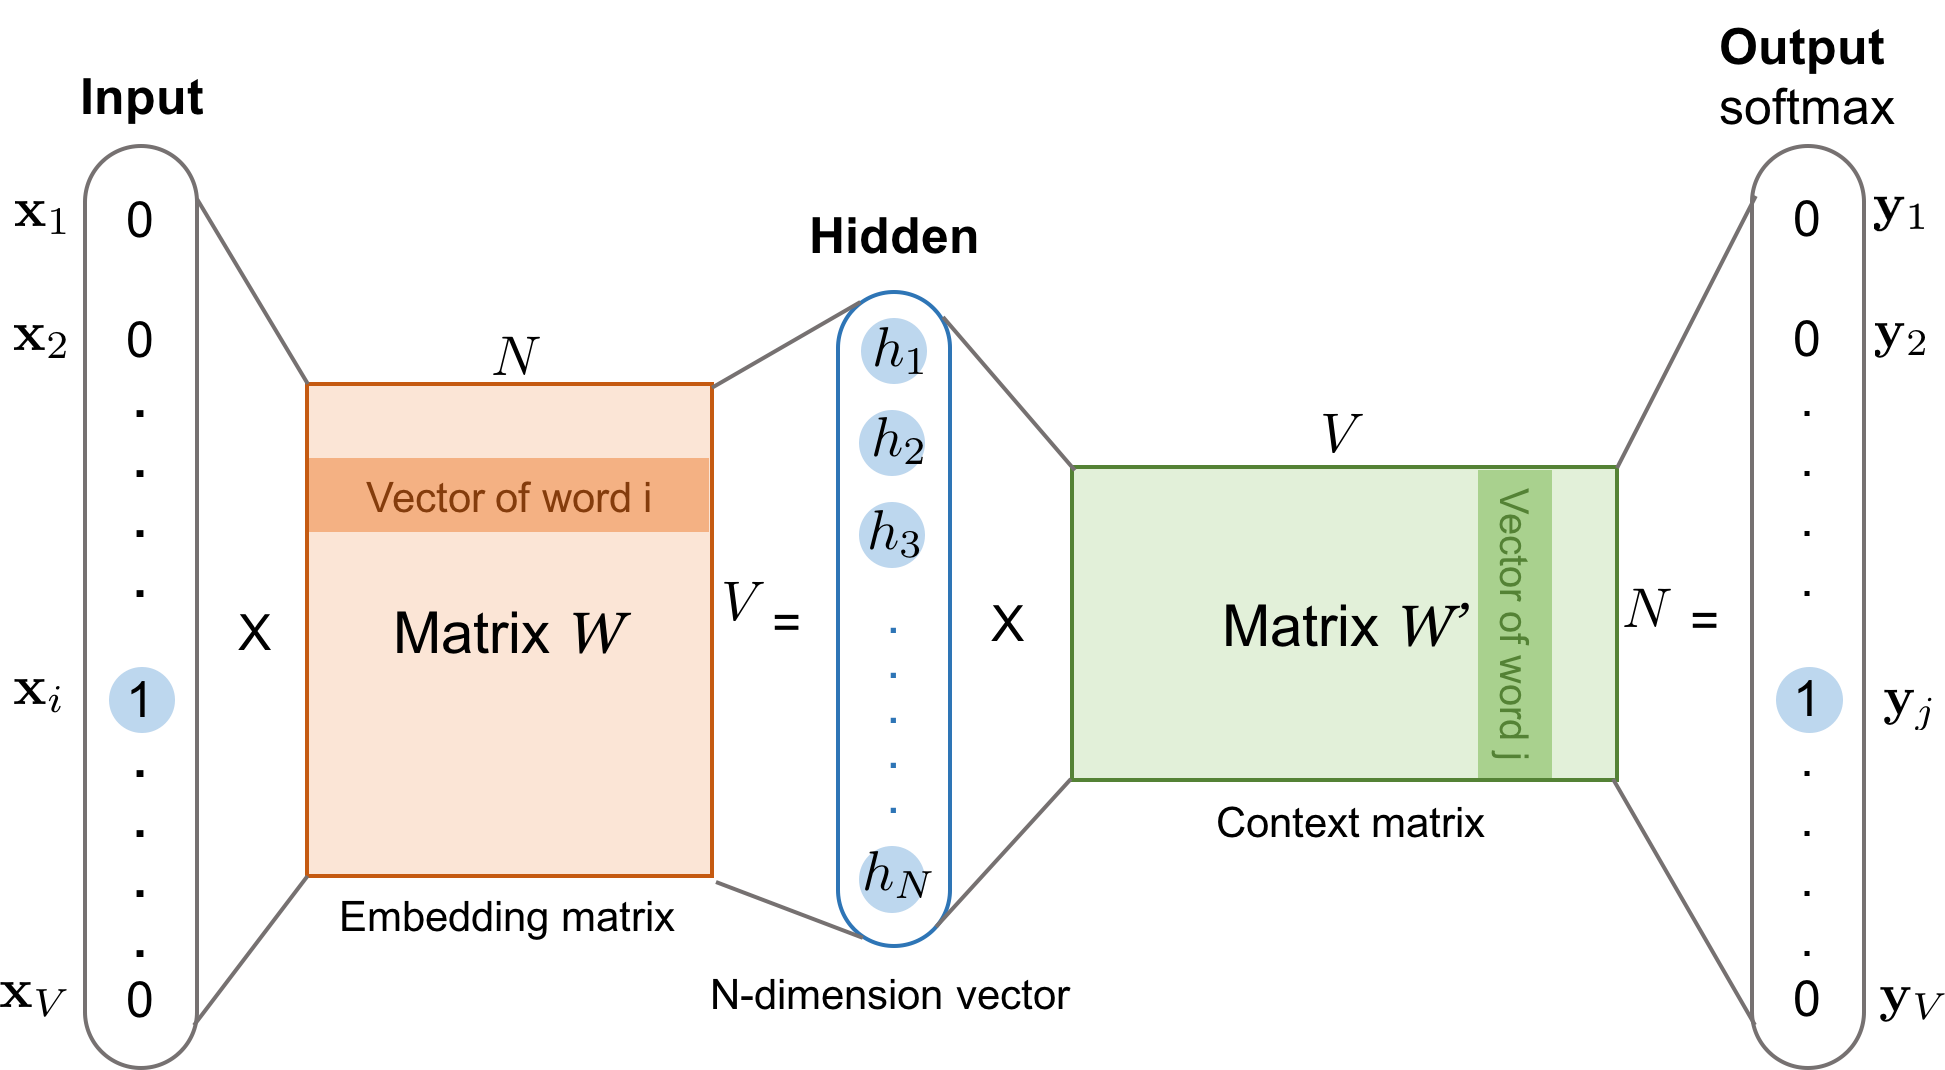
\includegraphics[width=0.7\textwidth]{imgs/skipgram_image.png}
    \vspace{-5pt}
    \caption{\tiny Skip-Gram Model; simplified version, with one input target word and one output context word. From \emph{Learning Word Embeddings}, by Lilian Weng, 2017. \url{https://lilianweng.github.io/lil-log/2017/10/15/learning-word-embedding.html}. Copyright n.d. by n.d.}
    \label{fig:SkipGram}
    \vspace{-5pt}
    \end{figure}
    
\end{frame}


\begin{frame}{Continuous-Bag-of-Words (CBOW)}\label{frame:CBOW}
    
    \begin{itemizeSpaced}{0pt}
        \item \textbf{Continuous bag of words model (CBOW)} is opposite of the Skip-Gram: predicts \emph{target} word based on a \emph{context} word. 
        
        \item Averages $n$ context words around target word $w_t$ to predict target (in hidden layer calculation): %\footnotemark 
        $
        \overrightarrow{h} 
        = \frac{1}{c} W \cdot \Big(\overrightarrow{x_1} + \overrightarrow{x_2} + ... + \overrightarrow{x_c} \Big) 
        = \frac{1}{c} \cdot \Big(\overrightarrow{v_{w_1}} + \overrightarrow{v_{w_2}} + ... + \overrightarrow{v_{w_c}} \Big)
        $
        
    \end{itemizeSpaced}
    
    \begin{figure}[h] 
    \vspace{-5pt}
    \centering
    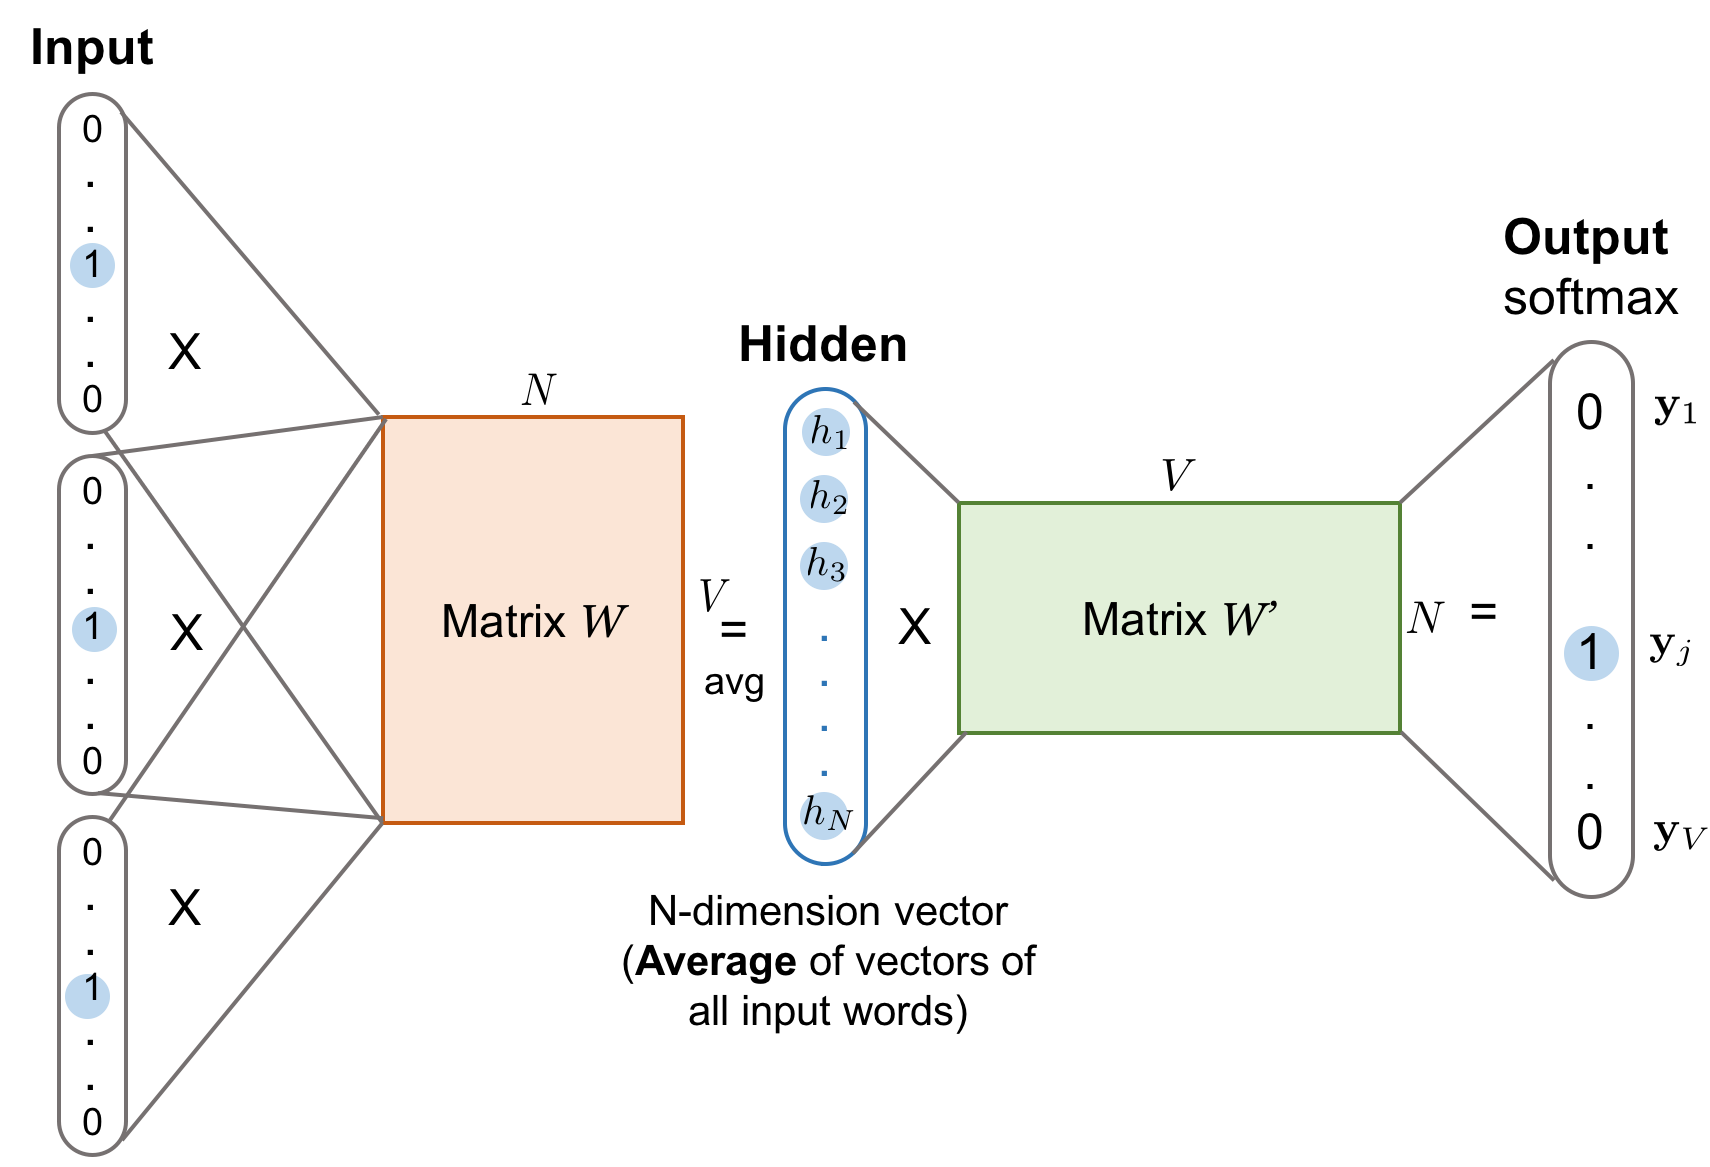
\includegraphics[width=0.7\textwidth]{imgs/cbow.png}
    \vspace{-5pt}
    \caption{\tiny CBOW Model with several one-hot encoded context words at the input layer and one target word at the output layer. From \emph{Learning Word Embeddings}, by Lilian Weng, 2017. \url{https://lilianweng.github.io/lil-log/2017/10/15/learning-word-embedding.html}}
    \label{fig:CBOW}
    \vspace{-5pt}
    \end{figure}
    
    %\footnotemark[1]{\footnotesize CBOW averaging distributional information of the context vectors makes it better suited for small datasets (Weng, 2018).}
    
\end{frame}



\begin{frame}{Phrase-Learning in Skip-Gram}

    \begin{itemizeSpaced}{7pt}
    
        \item \textbf{Problem with previous word vectors:} no \emph{phrase representation}
        \begin{itemize}
            \item “Canada” and “Air” in a phrase could not be recognized as part of a larger concept and thus combined into “Air Canada” (Mikolov et al., 2013a).
        \end{itemize}
        
        \item \textbf{Phrase-Skip-Gram Model}:
        \begin{itemizeSpaced}{2pt}
            \item uses \emph{unigram and bigram counts} to make phrases.
            
            \item ${\large S_{phrase} = \frac{C(w_i w_j) - \delta} {C(w_i)C(w_j)} }$ where $C(\cdot)$ = count of a unigram $w_i$ or bigram $w_i w_j$ and $\delta$ is a discounting threshold to avoid making infrequent words and phrases.
            
            \item Large $S_{phrase}$ indicates the \emph{phrase} is a phrase, less likely a bigram. 
        \end{itemizeSpaced}
        
        
        \item \textbf{Result: } linear structure \textbf{additive compositionality} of word vectors 
        
        \begin{itemize}
            \item \textbf{Explaining Additive Compositionality: }lets some individual words be combined into phrase and viewed as unique identity, while a bigram like “this is” should remain unchanged (Mikolov et al., 2013a, p. 5).
            
            \item \textbf{How It Occurs: } product of distributions in loss function acts like an ``and" function
        \end{itemize} 
        
        \begin{exampleBlock}{Additive Compositionality Example}
        
        If the phrase ``Volga River" appears numerously with ``Russian" and ``river" then: $vector(\texttt{"Russian"}) \! + \! vector(\texttt{"river"}) \; \Rightarrow \; vector(\texttt{"Volga River"})$
        
        \end{exampleBlock}
        
        
    \end{itemizeSpaced}
    
\end{frame}